\documentclass[french,11pt]{article}
\usepackage[utf8]{inputenc}
\usepackage[T1]{fontenc}
\usepackage{babel}
\usepackage{eurosym}
\usepackage[affil-it]{authblk}

\usepackage[table]{xcolor}

\usepackage{tikz}
\usetikzlibrary{arrows,decorations.markings}
\usetikzlibrary{cd}
\usetikzlibrary{shapes.geometric,fit}
\usetikzlibrary{positioning}

\usepackage{leadsheets}

\usepackage[top=4cm, bottom=4cm, left=3cm, right=3cm]{geometry}
\usepackage[fencedCode,inlineFootnotes,citations,definitionLists,hashEnumerators,smartEllipses,hybrid,pipeTables, tableCaptions]{markdown}
\usepackage{keyval}

\usepackage[backend=biber,style=alphabetic,citestyle=authoryear-comp]{biblatex}
\addbibresource{refs.bib}

\usepackage{minted}
\setkeys{Gin}{width=\linewidth,totalheight=\textheight,keepaspectratio}

\usepackage{mathtools}
\usepackage{amsmath}
\usepackage{amsfonts}
\usepackage{amsthm}
\usepackage{amssymb}



\usepackage{graphicx}
\graphicspath{{img/}}
\usepackage{wrapfig}
\usepackage{float}

\usepackage{hyperref}
\interfootnotelinepenalty=10000

\usepackage{setspace}
\onehalfspacing

\usepackage{caption}
\usepackage{subcaption}
\tikzcdset{every label/.append style = {font = \tiny}}

\usepackage{csquotes}
\usepackage{comment}


\usepackage{tabularx}
\definecolor{tableShade}{gray}{0.9}

\usepackage[shortlabels]{enumitem}





\title{LiveScaler}
\author{Alice Rixte}
\begin{document}
\maketitle

\tableofcontents

\section{Introduction}

\section{Transformations de gammes}
\begin{comment}
  \subsection{Quelles transformations de gamme autoriser ?}
Les transformation affines de la forme $an + b$ où $n$ est la note de départ.
\subsection{Pourquoi ces transformations ?}
\begin{enumerate}
  \item Ces transformations sont adaptées à la musique tonale occidentale : passage du majeur au mineur.
  \item Elles sont facilement implémentables
  \item Elles peuvent être exprimées par une paire d'entiers, ce qui permet de les communiquer directement via MIDI.
\end{enumerate}


\subsection{Peut-on quand même sortir de la tonalité ?}
Oui : \begin{enumerate}
  \item on peut passer d'une gamme quelconque à une gamme par tons
  \item elles s'appliquent dans un contexte microtonal
  \item Possibilité d'ajouter une permutation quelconque personnalisée
\end{enumerate} 
\end{comment}

Nous définissons ici une \emph{transformation de gamme} comme une fonction qui à toute hauteur de note associe une nouvelle hauteur de note a priori quelconque, autrement dit une fonction $\mathbb{Z}$ dans $\mathbb{Z}$. Un bon exemple de transformation de gamme est la transposition : à chaque note $n$ on associe la note $n+\tau$  décalée de $\tau$ demi-tons vers l'aigu lorsque $\tau$ est positif et vers le grave lorsque $\tau$ est négatif. Ainsi, une transposition de $\tau$ demi-tons est représentée par la transformation de gamme $ n \mapsto n+\tau$ (voir Figure \ref{fig:transp}).


\subsection{Transformations affines}

Les transformations de gamme qui vont nous intéresser ici sont les \emph{transformation affines}\footnote{Cette définition est inspirée par les automorphismes du groupe $T/I$ présentés par \textcite{lewin1990klumpenhouwer}.}, c'est-à-dire les fonctions de la forme $A\langle\mu,\tau\rangle : n \mapsto \mu n + \tau$ avec $\mu$ le \emph{coefficient modal} de la transformation affine et $\tau$ le \emph{coefficient de transposition}. 

Les transformations affines ont la propriété importante de préserver les classes de hauteur \footnote{En effet, pour toute base $b\in \mathbb{N}^*$, $\forall n_1,n_2 \in \mathbb{Z}, n_1 \equiv n_2 \mod b \implies \mu n_1 + \tau \equiv \mu n_2 + \tau \mod b$. Avec $b=12$, on obtient le résultat pour les classes de hauteurs dodécaphoniques. }  (au sens de \cite{forte1973structure}) c'est-à-dire que si deux notes sont identiques à l'octave près, alors elles le seront toujours une fois la transformation affine appliquée. 

Nous allons à présent étudier plusieurs exemples afin de donner au lecteur un aperçu de leur expressivité.
\subsubsection{Transpositions}
\begin{figure}[htbp]
  \centering
  \begin{tikzpicture}[baseline= (a).base]    

    \node[scale=1] (a) at (0,0){
    \begin{tikzcd}[column sep=0pt, minimum width=11.5mm, row sep=0.1cm]
    {...} & {A_{-1}} & {A\sharp_{-1}} & {B_{-1}} & {C_{0}} & {C\sharp_{0}} & {D_0} & {D\sharp_0} & {E_0} & {F_0} & {F\sharp_0} & {G_0} & {...} \\
    {...} & {-3} & {-2} & {-1} & 0 & 1 & 2 & 3 & 4 & 5 & 6 & 7 & {...} \\
    {} &&&&&&&&&&& {} \\
    {} &&&&&&&&&&& {} \\
    {} &&&&&&&&&&& {} \\
    {} &&&&&&&&&&& {} \\
    {} &&&&&&&&&&& {} \\
    {} &&&&&&&&&&& {} \\
    {...} & {-3} & {-2} & {-1} & 0 & 1 & 2 & 3 & 4 & 5 & 6 & 7 & {...} \\
    {...} & {A_{-1}} & {A\sharp_{-1}} & {B_{-1}} & {C_0} & {C\sharp_0} & {D_0} & {D\sharp_0} & {E_0} & {F_0} & {F\sharp_0} & {G_0} & {...}
    \arrow[color={rgb,255:red,117;green,117;blue,117}, dotted, from=2-1, to=9-3]
    \arrow[from=2-2, to=9-4]
    \arrow[from=2-3, to=9-5]
    \arrow[from=2-4, to=9-6]
    \arrow[from=2-5, to=9-7]
    \arrow[from=2-6, to=9-8]
    \arrow[from=2-7, to=9-9]
    \arrow[from=2-8, to=9-10]
    \arrow[from=2-9, to=9-11]
    \arrow[from=2-10, to=9-12]
    \arrow[color={rgb,255:red,117;green,117;blue,117}, dotted, from=2-11, to=9-13]
    \end{tikzcd}
  };
  \end{tikzpicture}
  \caption{La transformation $A \langle 1,2 \rangle : n \mapsto n + 2$ correspond à la  transposition d'un ton vers l'aigu}\label{fig:transp}
\end{figure}
Lorsque $\mu = 1$, les transformations affines $A\langle 1,\tau \rangle : n \mapsto n + \tau$ permettent de représenter toutes les transpositions possibles (voir Figure \ref{fig:transp}).


\subsubsection{Inversions}

\begin{figure}[htbp]
  \centering
  \begin{tikzpicture}[baseline= (a).base]

    \node[scale=1] (a) at (0,0){
      \begin{tikzcd}[column sep=0mm, minimum width = 0mm, minimum height=7mm, row sep=0cm]
        \svdots   & \svdots & \hspace{20mm} & \svdots & \svdots \\
        \writechord{G}_{5}  & 7  & & 7  & \writechord{G}_{5}  \\
        \writechord{F#}_{5} & 6  & & 6  & \writechord{F#}_{5} \\
        \writechord{F}_{5}  & 5  & & 5  & \writechord{F}_{5}  \\
        \writechord{E}_{5}  & 4  & & 4  & \writechord{E}_{5}  \\
        \writechord{D#}_{5} & 3  & & 3  & \writechord{D#}_{5} \\
        \writechord{D}_{5}  & 2  & & 2  & \writechord{D}_{5}  \\
        \writechord{C#}_{5} & 1  & & 1  & \writechord{C#}_{5} \\
        \writechord{C}_{5}  & 0  & & 0  & \writechord{C}_{5}  \\
        \writechord{B}_{4}  & -1 & & -1 & \writechord{B}_{4}  \\
        \writechord{A#}_{4} & -2 & & -2 & \writechord{A#}_{4} \\
        \writechord{A}_{4}  & -3 & & -3 & \writechord{A}_{4}  \\
        \svdots         & \svdots & & \svdots &         \svdots 
        \arrow[from=2-2, to=12-4]
        \arrow[from=4-2, to=10-4, color={rgb,255:red,117;green,117;blue,117}, dashed]
        \arrow[from=5-2, to=9-4]
        \arrow[from=7-2, to=7-4, color={rgb,255:red,117;green,117;blue,117}, dashed]
        \arrow[from=9-2, to=5-4]
        \arrow[from=10-2, to=4-4, color={rgb,255:red,117;green,117;blue,117}, dashed]
        \arrow[from=12-2, to=2-4]
      \end{tikzcd}
    };
  \end{tikzpicture}
  \caption{La transformation $A\langle -1,4\rangle :n\mapsto -n + 4$ avec $\alpha =$ \writechord{C}$_5$ et $\beta = 12$}
  \medskip
  \small
  Pour des raisons de lisibilité seules les flèches de la gamme de Do majeur ont été tracées. On notera la passage de l'accord \writechord{Cma} à \writechord{Ami} et de \writechord{Ami} à \writechord{Cma}.
  \label{fig:inversion}
\end{figure}

\begin{figure}
  %\centering
  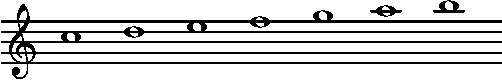
\includegraphics[width=\columnwidth]{c-maj-crop.pdf}
  \begin{tabularx}{\columnwidth}{ YYYYZ }
    &&$ \mathlarger{\mathlarger{\mathlarger{\mathlarger\Downarrow}}}$ & $A\langle -1,4 \rangle$&
    \end{tabularx}
  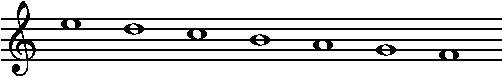
\includegraphics[width=\columnwidth]{e-mod-crop.pdf}
  \caption{L'image de la gamme de Do majeur par $A\langle -1,4 \rangle$ est un mode de Mi}
  \label{fig:modeE}
\end{figure}

Lorsque $\mu = -1$, les transformations $A \langle -1,\tau\rangle : n\mapsto -n + \tau$ permettent de passer d'une gamme majeure à un mode de Mi et réciproquement (voir Figure \ref{fig:modeE}). La Figure \ref{fig:inversion} illustre la manière dont la triade \writechord{C}$_5$, \writechord{E}$_5$, \writechord{G}$_5$ est  par $A\langle -1,4 \rangle$ en la triade \writechord{E}$_5$, \writechord{C}$_5$, \writechord{A}$_4$. De même, l'image de la triade \writechord{A}$_4$, \writechord{C}$_5$, \writechord{E}$_5$  est  \writechord{G}$_5$, \writechord{E}$_5$, \writechord{G}$_5$. Comme les transformations affines préservent les classes de hauteur, on peut affirmer plus généralement que $A \langle -1,4\rangle$ transforme l'accord \writechord{Cma} en \writechord{Ami}   et \writechord{Ami} en \writechord{Cma}. 

Remarquons de plus qu'en changeant l'ancre,  en choisissant $\alpha =$  \writechord{G}$_4$ par exemple, l'image de l'accord \writechord{Gma} par $A\langle-1,4 \rangle$ sera \writechord{Emi}. La Table \ref{tab:triadesA-14} explicite les images des accords de la gamme de Do majeur par $A\langle -1,4 \rangle$ lorsque $\alpha = $ \writechord{C}$_n$ et des accords de la gamme de Sol majeur lorsque l'on change l'ancre pour $\alpha =$ \writechord{G}$_n$, avec $n$ un entier quelconque.


\begin{table}[htbp]
  
  \centering % instead of \begin{center}
  \begin{tabular}{cccccccc}
      \writechord{Cma} & $\mapsto$ & \writechord{Ami} & & & \writechord{Gma} & $\mapsto$ & \writechord{Emi}\\
      \writechord{Dmi} & $\mapsto$ & \writechord{Gma} & & & \writechord{Ami} & $\mapsto$ & \writechord{Dma}\\
      \writechord{Emi} & $\mapsto$ & \writechord{Fma} & & & \writechord{Bmi} & $\mapsto$ & \writechord{Cma}\\
      \writechord{Fma} & $\mapsto$ & \writechord{Emi} & & & \writechord{Cma} & $\mapsto$ & \writechord{Bmi}\\
      \writechord{Gma} & $\mapsto$ & \writechord{Dmi} & & & \writechord{Dma} & $\mapsto$ & \writechord{Ami}\\
      \writechord{Ami} & $\mapsto$ & \writechord{Cma} & & & \writechord{Emi} & $\mapsto$ & \writechord{Gma}\\
      \writechord{Bo} & $\mapsto$ & \writechord{Bo} & & & \writechord{F#o} & $\mapsto$ & \writechord{F#o}
  \end{tabular}
  \caption{Images des accords de la gamme de Do majeur par $A\langle -1, 4 \rangle$ pour $\alpha =$ \writechord{C}$_n$ (à gauche) et de la gamme de Sol majeur pour $\alpha =$ \writechord{G}$_n$ (à droite), pour $n\in\mathbb{Z}$} 
  \label{tab:triadesA-14}
\end{table}

Ainsi, en se basant sur l'image de l'accord majeur dont la tonique correspond à l'ancre, nous pouvons associer les transformations affines pour lesquelle $\mu = 1$ ou $\mu=-1$ au degré de l'image de cet accord dans la gamme. Par exemple, $A\langle -1,4 \rangle$ peut être associée au degré \writechord{vi} car elle associe le sixième degré mineur à  l'accord majeur dont la tonique est l'ancre (\writechord{Ami} pour \writechord{Cma}, \writechord{Emi} pour \writechord{Gma}, \dots). On obtient ainsi une notation plus intuitive que la notation mathématique, dont la table \ref{tab:degrees} donne un aperçu. 

\begin{table}[htbp]
  \centering
  \rowcolors{2}{gray!25}{white}
  \begin{tabular}{ccc}
    \rowcolor{gray!50}
    Degré & Transformation affine\\
    \writechord{I} & $A\langle ~~1, ~~0\rangle$\\
    \writechord{ii} &  $A\langle -1, -3 \rangle$\\
    \writechord{iii} &  $A\langle -1, -1 \rangle$\\
    \writechord{IV} &  $A\langle ~~1,~~ 5 \rangle$\\
    \writechord{V} &  $A\langle ~~ 1, ~~7 \rangle$\\
    \writechord{vi}& $A\langle -1, ~~4\rangle$\\
    \writechord{vii} & $A\langle -1, ~~6 \rangle$\\
  \end{tabular}
  \caption{ Correspondances entre triades d'une gamme majeure et transformations de gamme\label{tab:degrees} } 
\end{table}

Remarquons que, de manière générale, les inversions affines se comportent moins bien sur les modes non naturels. Par exemple, $A\langle -1, 4\rangle ($\writechord{G\sharp}$) = $ \writechord{G\sharp} donc l'image de la gamme de La mineur harmonique par $A\langle -1, 4\rangle$ contient les notes \writechord{C}, \writechord{D}, \writechord{E}, \writechord{F}, \writechord{G}, \writechord{G\sharp}, \writechord{B}, ce qui ne correspond pas à un mode standard de la musique tonale. C'est une des faiblesses des transformations affines.

\subsubsection{Transformation vers une gamme par ton}
Lorsque $\mu = 2$ ou $\mu = -2$, les transformations affines envoient n'importe quelle gamme vers une gamme apparentée à une gamme par tons (voir Figure \ref{fig:gammepartons}). Les transformations affines peuvent donc permettre de sortir du cadre de la musique tonale occidentale.

\begin{figure}[htbp]
  \centering
  \begin{tikzpicture}[baseline= (a).base]    

    \node[scale=1] (a) at (0,0){
    \begin{tikzcd}[column sep=0pt, minimum width=11.5mm, row sep=0.1cm]
    \dots & G_{-2} & G\sharp_{-2} & A_{-2} & A\sharp_{-2} & B_{-2} & C_{-1} & C\sharp_{-1} & D_{-1} & D\sharp_{-1} & E_{-1} & F_{-1}  & \dots \\
      \dots & -5 &-4 & -3 & -2 & -1 & 0 & 1 & 2 & 3 & 4 & 5 &  \dots \\
      {} &&&&&&&&&&& {} \\
      {} &&&&&&&&&&& {} \\
      {} &&&&&&&&&&& {} \\
      {} &&&&&&&&&&& {} \\
      {} &&&&&&&&&&& {} \\
      {} &&&&&&&&&&& {} \\
      \dots & -5 &-4 & -3 & -2 & -1 & 0 & 1 & 2 & 3 & 4 & 5 &  \dots \\
      \dots & G_{-2} & G\sharp_{-2} & A_{-2} & A\sharp_{-2} & B_{-2} & C_{-1} & C\sharp_{-1} & D_{-1} & D\sharp_{-1} & E_{-1} & F_{-1} & \dots \\
      \arrow[color={rgb,255:red,117;green,117;blue,117}, dotted, from=2-4, to=9-1]
      \arrow[from=2-5, to=9-3]
      \arrow[from=2-6, to=9-5]
      \arrow[from=2-7, to=9-7]
      \arrow[from=2-8, to=9-9]
      \arrow[from=2-9, to=9-11]
      \arrow[color={rgb,255:red,117;green,117;blue,117}, dotted,from=2-10, to=9-13]
      %\arrow[color={rgb,255:red,117;green,117;blue,117}, dotted, from=2-11, to=9-15]
      %\arrow[from=2-9, to=9-3]
      %\arrow[from=2-10, to=9-3]
    \end{tikzcd}
    };
  \end{tikzpicture}   
  \caption{La transformation $A\langle 2,0\rangle :n\mapsto 2n$ permet d'obtenir des gammes apparentées à la gamme par tons.\label{fig:gammepartons}}
\end{figure}

Contrairement aux inversions et aux transpositions, cette transformation n'est pas bijective : l'image de $A\langle 2,0 \rangle$ contient exactement $6$ classes de hauteurs qui correspondent aux $6$ notes d'une des deux gammes par tons. Il est intéressant de noter que l'image d'une gamme majeure ou mineure naturelle par $A\langle 2,\tau\rangle$ contient les $6$ notes de la gamme par tons (voir Table \ref{tab:minparton}). Ce n'est pas le cas pour la gamme mineure harmonique dont l'image par $A\langle 2,\tau\rangle$ ne contient que $5$ classes de hauteur.




\begin{table}[htbp]
  \centering
  \begin{subtable}{0.45\textwidth}
    \centering % instead of \begin{center}
      \begin{tabular}{ccc}
          \writechord{C} & $\mapsto$ & \writechord{C}\\
          \writechord{D} & $\mapsto$ & \writechord{E}\\
          \writechord{E} & $\mapsto$ & \writechord{G\sharp}\\
          \writechord{F} & $\mapsto$ & \writechord{A\sharp}\\
          \writechord{G} & $\mapsto$ & \writechord{D}\\
          \writechord{A} & $\mapsto$ & \writechord{F\sharp}\\
          \writechord{B} & $\mapsto$ & \writechord{A\sharp}
      \end{tabular}
  \end{subtable}
  \begin{subtable}{0.45\textwidth}
      \centering % instead of \begin{center}
      \begin{tabular}{ccc}
          \writechord{C} & $\mapsto$ & \writechord{C}\\
          \writechord{D} & $\mapsto$ & \writechord{E}\\
          \writechord{E\flat} & $\mapsto$ & \writechord{F\sharp}\\
          \writechord{F} & $\mapsto$ & \writechord{A\sharp}\\
          \writechord{G} & $\mapsto$ & \writechord{D}\\
          \writechord{A\flat} & $\mapsto$ & \writechord{E}\\
          \writechord{B\flat} & $\mapsto$ & \writechord{G\sharp}
      \end{tabular}
    \end{subtable}
    \caption{Image des gammes de Do majeur (à gauche) et Do mineur (à droite) par $A\langle 2, 0 \rangle$\label{tab:minparton}}
\end{table}
\subsubsection{Coefficient modal}

La Table \ref{tab:classmu} résume les différents types de transformations qu'offrent les transformations affines, ainsi que le nombre de classes de hauteur dans l'image de ces transformations \footnote{On montre aisément que le nombre de classes de hauteur dans l'image de $A\langle \mu, \tau\rangle$ est égal à $\frac{12}{\mu\wedge 12}$ où $\wedge$ dénote le pgcd de deux entiers.}. Les transformations affines bijectives - leur image contient $12$ classes de hauteurs - correspondent  aux automorphismes $F\langle u,j \rangle$ du groupe $T/I$ décrits par \cite{lewin1990klumpenhouwer}.


\begin{table}[h]
  \centering
  \rowcolors{2}{gray!25}{white}
  \begin{tabular}{ccc}
    \rowcolor{gray!50}
    $\mu$ & Type de transformation & Classes de hauteur\\
    -1 & Inversions majeur/mineur & 12\\
    0 & Octaves & 1\\
    1 & Transpositions & 12 \\
    -2,2 & Gamme par tons & 6 \\
    -3,3 & Tierces mineures &4 \\
    -4,4 & Tierces majeures & 3\\
    -5,5 & $F\langle 5,\tau \rangle$, $F\langle 7,\tau \rangle$& 12 \\
    -6,6 & Tritons & 2\\
  \end{tabular}
  \caption{Classification des transformations affines en fonction de leur coefficient modal $\mu$\label{tab:classmu} } 
\end{table}
\subsection{Restriction de l'écart de hauteur}

\section{Implémentation des transformations de gamme : LiveScaler}
\subsection{Justification du choix M4L /Ableton Live}
\begin{enumerate}
  \item Outil populaire dans le domaine de l'EDM
  \item Facilité d'utilisation et intégration dans un environnement 
  \item Prototypage aisé dans M4L
  \item Communication entre les entités d'Ableton Live via messages M4L
\end{enumerate}
\subsection{Comment appliquer la transformation ?}
Architecture chef d'orchestre/ instrument : 
\begin{enumerate}
  \item Un seul changement de gamme est envoyé à tous les instruments simultanément
  \item Chaque instrument applique la transformation selon ses propres paramètres (e.g. intervalle de repliement)
  \item Deux types de paramètres : \begin{itemize}
    \item Paramètres globaux envoyés sous la forme de messages à tous les instruments sous forme de message.
    \item Paramètre propre à chaque instrument d'interprétation des messages reçus.
    \end{itemize}
\end{enumerate}

\subsection{Quand appliquer la transformation ? }
Instantanément, car le flux MIDI en entrée fait office de "quantize".  ===> Quid des notes en cours ?
\begin{enumerate}
  \item On les arrête
  \item Legato
  \item Retrigger
\end{enumerate}
===> Le choix se fait séparément pour chaque instrument

\subsection{Comment éviter que les notes soient trop aiguës ou trop graves ?}
Repliement des transformation de gamme sur un intervalle
\begin{enumerate}
  \item Limiter l'écart de hauteur entre la note initiale et la note après la transformation.
  \item Possibilité d'adapter le repliement au morceau
\end{enumerate}
===> le choix se fait séparément pour chaque instrument
\section{Performance live avec LiveScaler}

\section{Travaux connexes}
\subsection{Transformations de gamme en live coding}
\begin{enumerate}
  \item propositions de Tidal
  \item algorave
\end{enumerate}
\subsection{Théorie transformationnelle}
\begin{enumerate}
  \item Les transformations affines sont une généralisation 
  \begin{enumerate}
    \item des Tonnetz
    \item des k-Nets
  \end{enumerate}
  \item ces transformations sont étudiées et utilisées surtout dans un contexte d'analyse et d'aide à la composition (OpenMusic)
\end{enumerate}

\subsection{Macro contrôle d'un morceau de musique électronique}
\begin{enumerate}
  \item "Changing musical emotion"
\end{enumerate}

\section{Conclusion}

\section{Annexe : mapping de LiveScaler}

\newpage
\printbibliography

\end{document}
